% Auto-generated by r_project/results/step5_diagnostics.R at commit 731ea2f (uncommitted changes)

\begin{figure}[htbp]
\centering
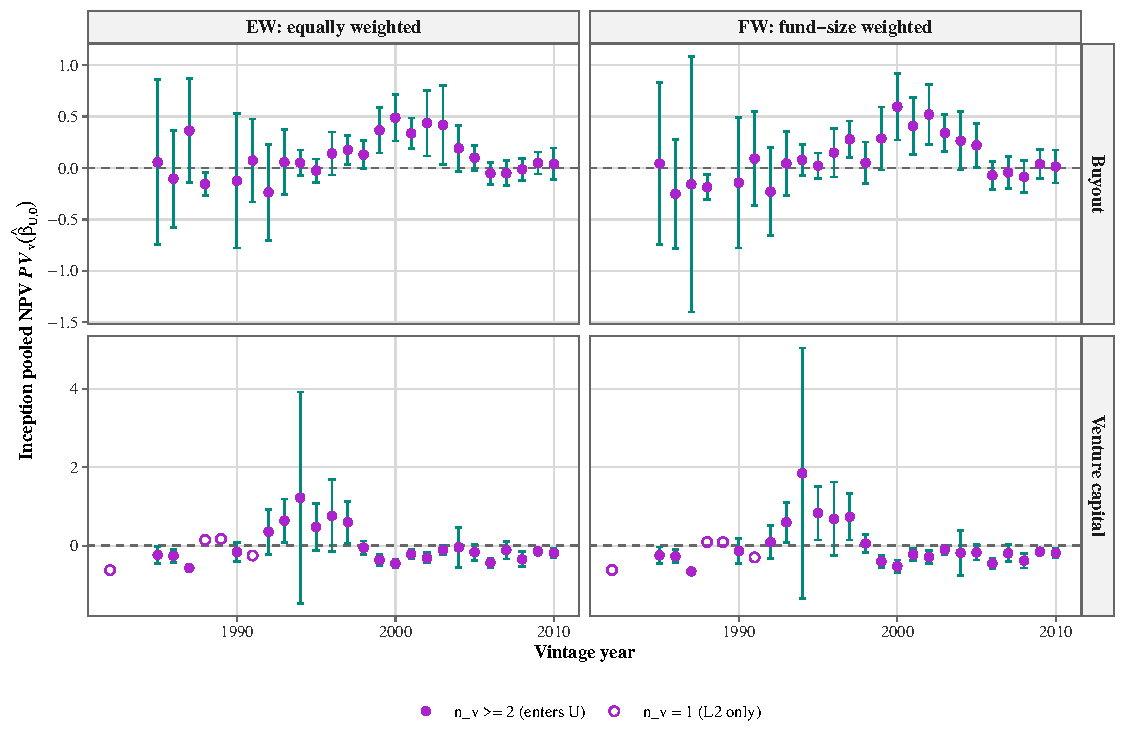
\includegraphics[width=0.92\textwidth]{figure_S5_vintage_residuals.pdf}
\caption{Vintage-level inception pricing errors $PV_v(\hat\beta_{U,0})$ with within-vintage $\pm1.96\,\mathrm{SE}$ bars}
\label{fig:vintage_residuals}
\par\vspace{2pt}
{\scriptsize\textit{Notes:} North America complete-history sample ($V\le 2010$). Each point is the constant-composition vintage portfolio inception NPV evaluated at the headline $U_{v,0}$ ($q_v=1$) single-factor estimate $\hat\beta_{U,0}$. Vertical bars show $\pm 1.96$ within-vintage standard errors of the weighted fund mean for vintages with $n_v\ge 2$ funds; open circles mark singleton vintages ($n_v=1$, entering L2 only). Persistent multi-vintage deviations (notably VC 1993--1997) visually separate vintage-level cohort realizations from within-vintage idiosyncratic dispersion.}
\end{figure}
